\chapter{Pomiary}
Rozdział ten ma za zadanie opisać pomiary dokonane
za pomocą czujnika klimatycznego realizowanego
w~tym projekcie.

\section{Przygotowanie do pomiarów}
Dla wygody użytkowania czujnik oraz kondensatory zostały 
zamontowane na ramie stworzonej w~technologii druku 3D,
widocznej na rysunku~\ref{rys:frame}.
Rysunek~\ref{rys:pcb_on_frame} przedstawia płytkę drukowaną 
przymocowaną do ramy,
uzupełnioną o~moduły pomiarowe, nadajnik radiowy oraz
diodę statusu. Dioda została podpięta do linii zasilania
nieużywanej magistrali 1--Wire.

\begin{figure}[H]
    \centering
    \begin{minipage}{0.45\textwidth}
        \centering
        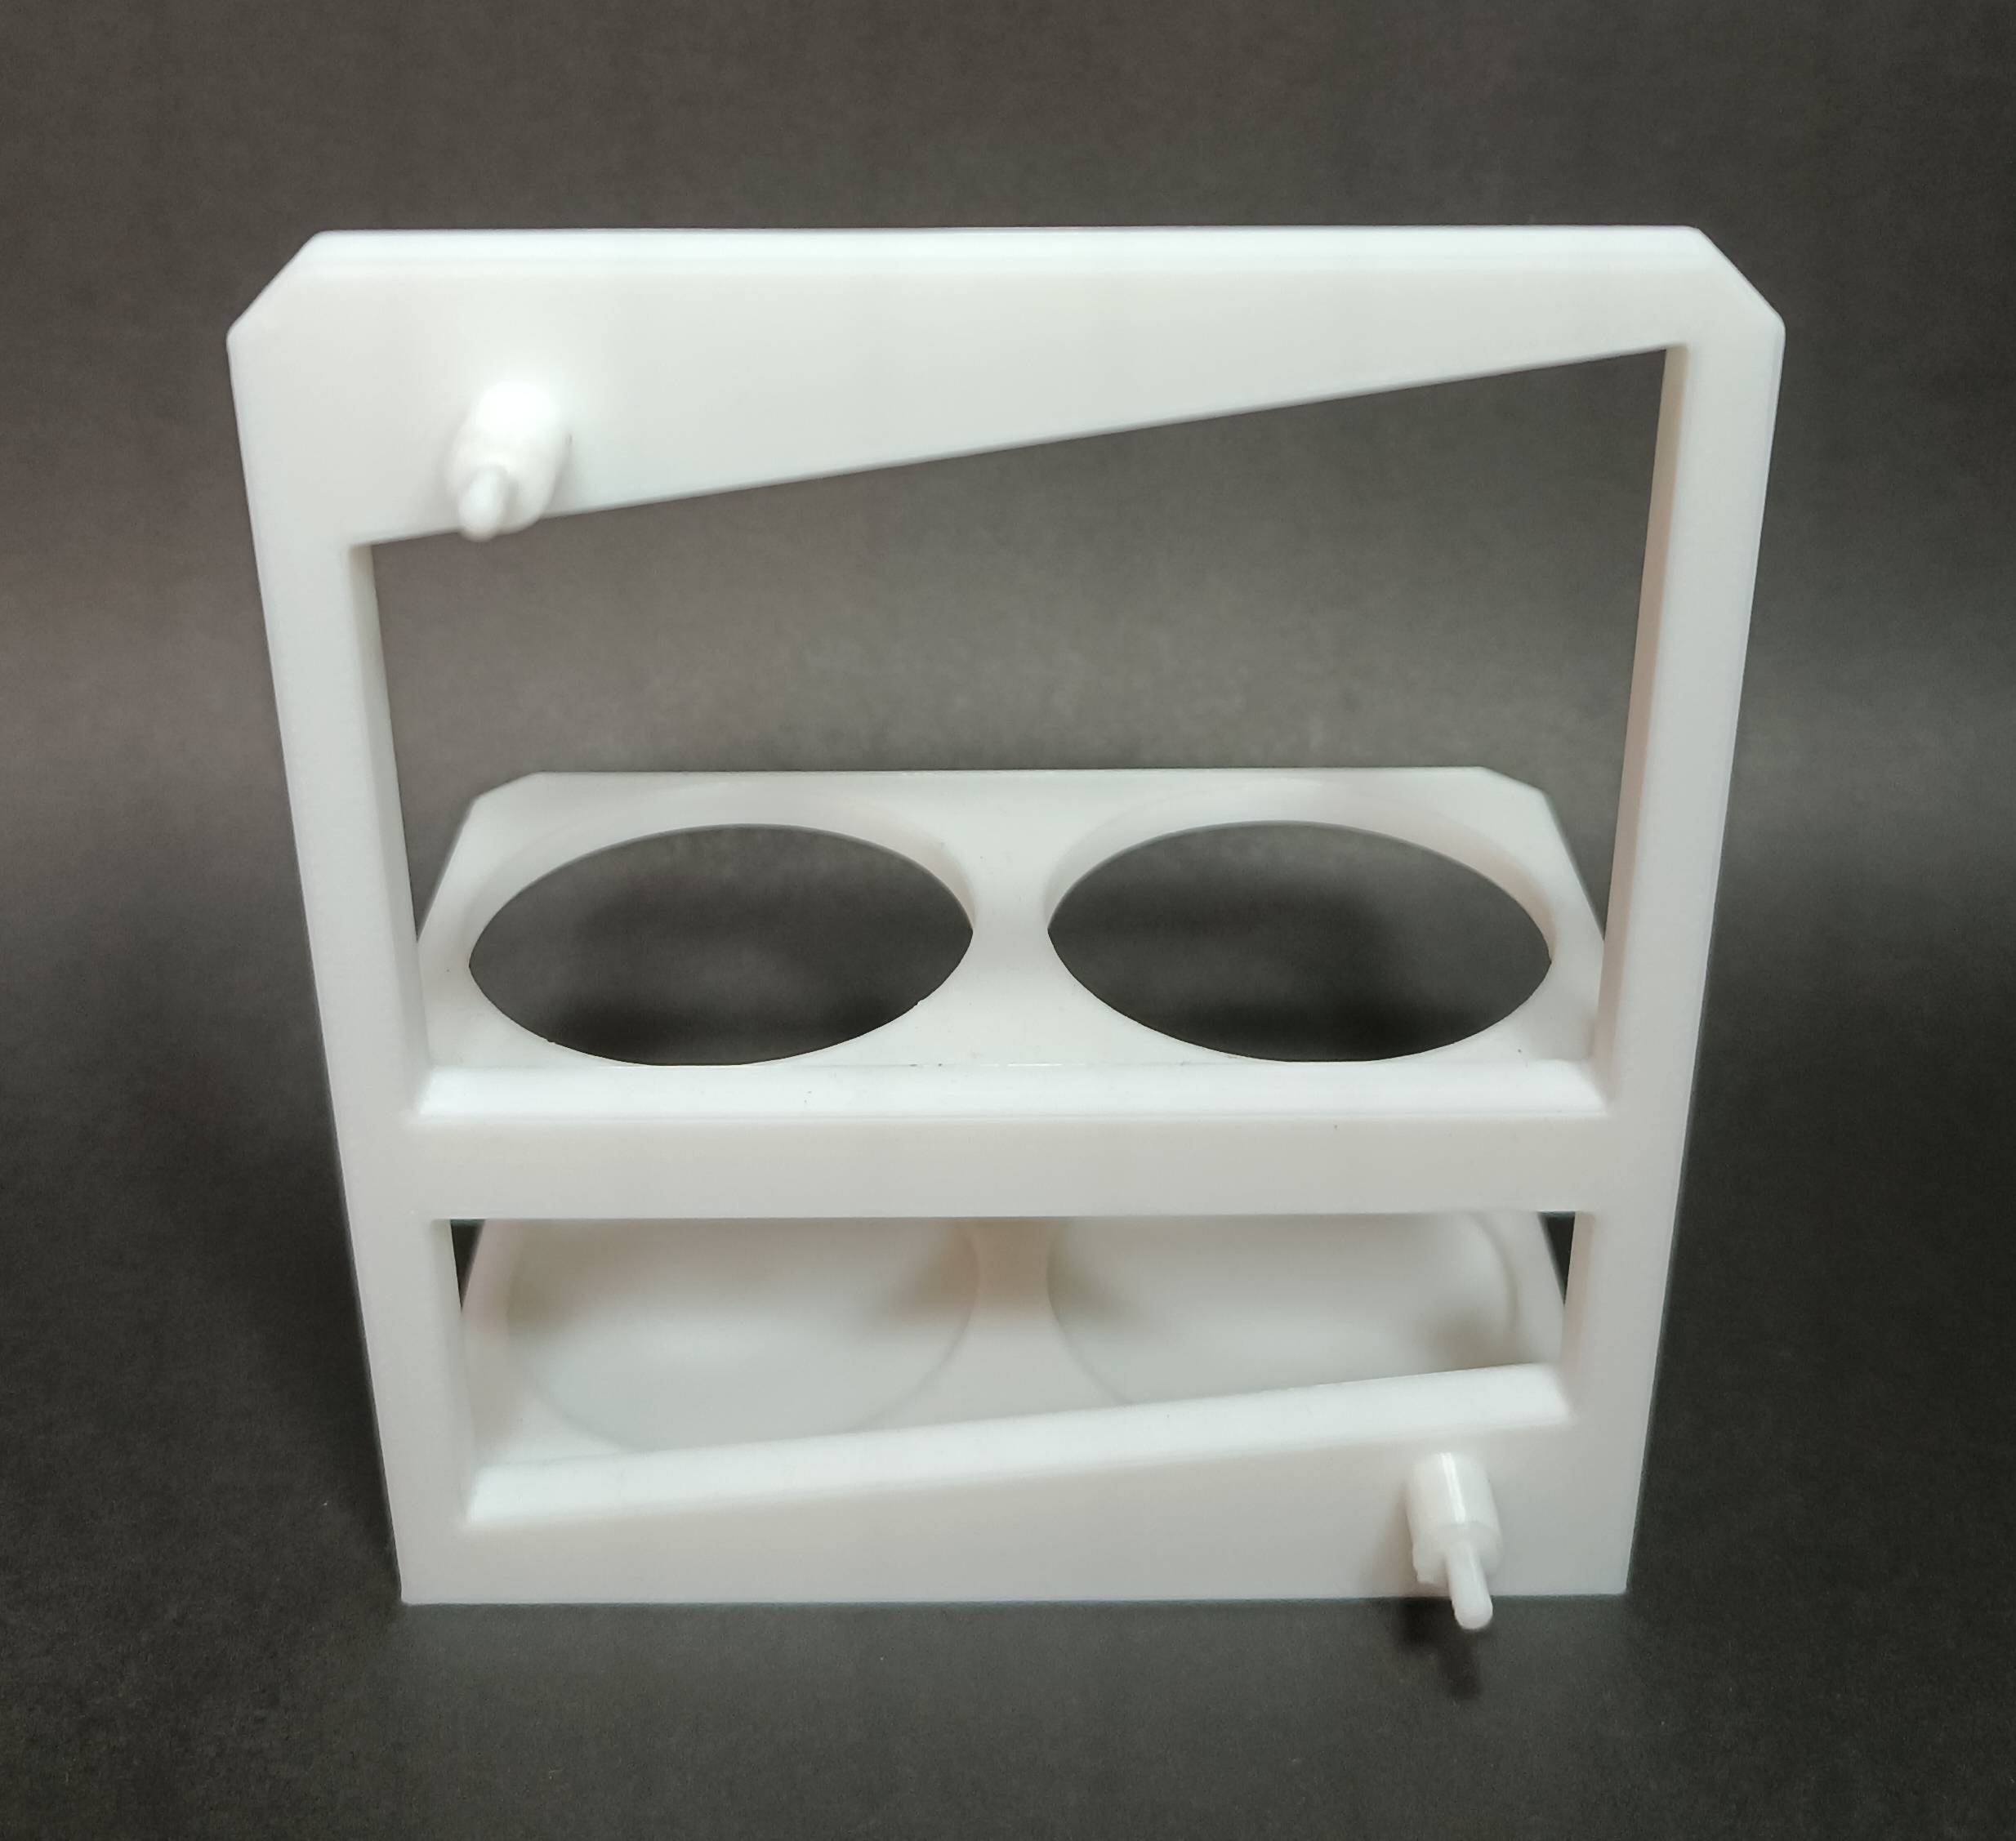
\includegraphics[width=0.9\textwidth]{fig/img/frame_front.png}
    \end{minipage}\hfill
    \begin{minipage}{0.45\textwidth}
        \centering
        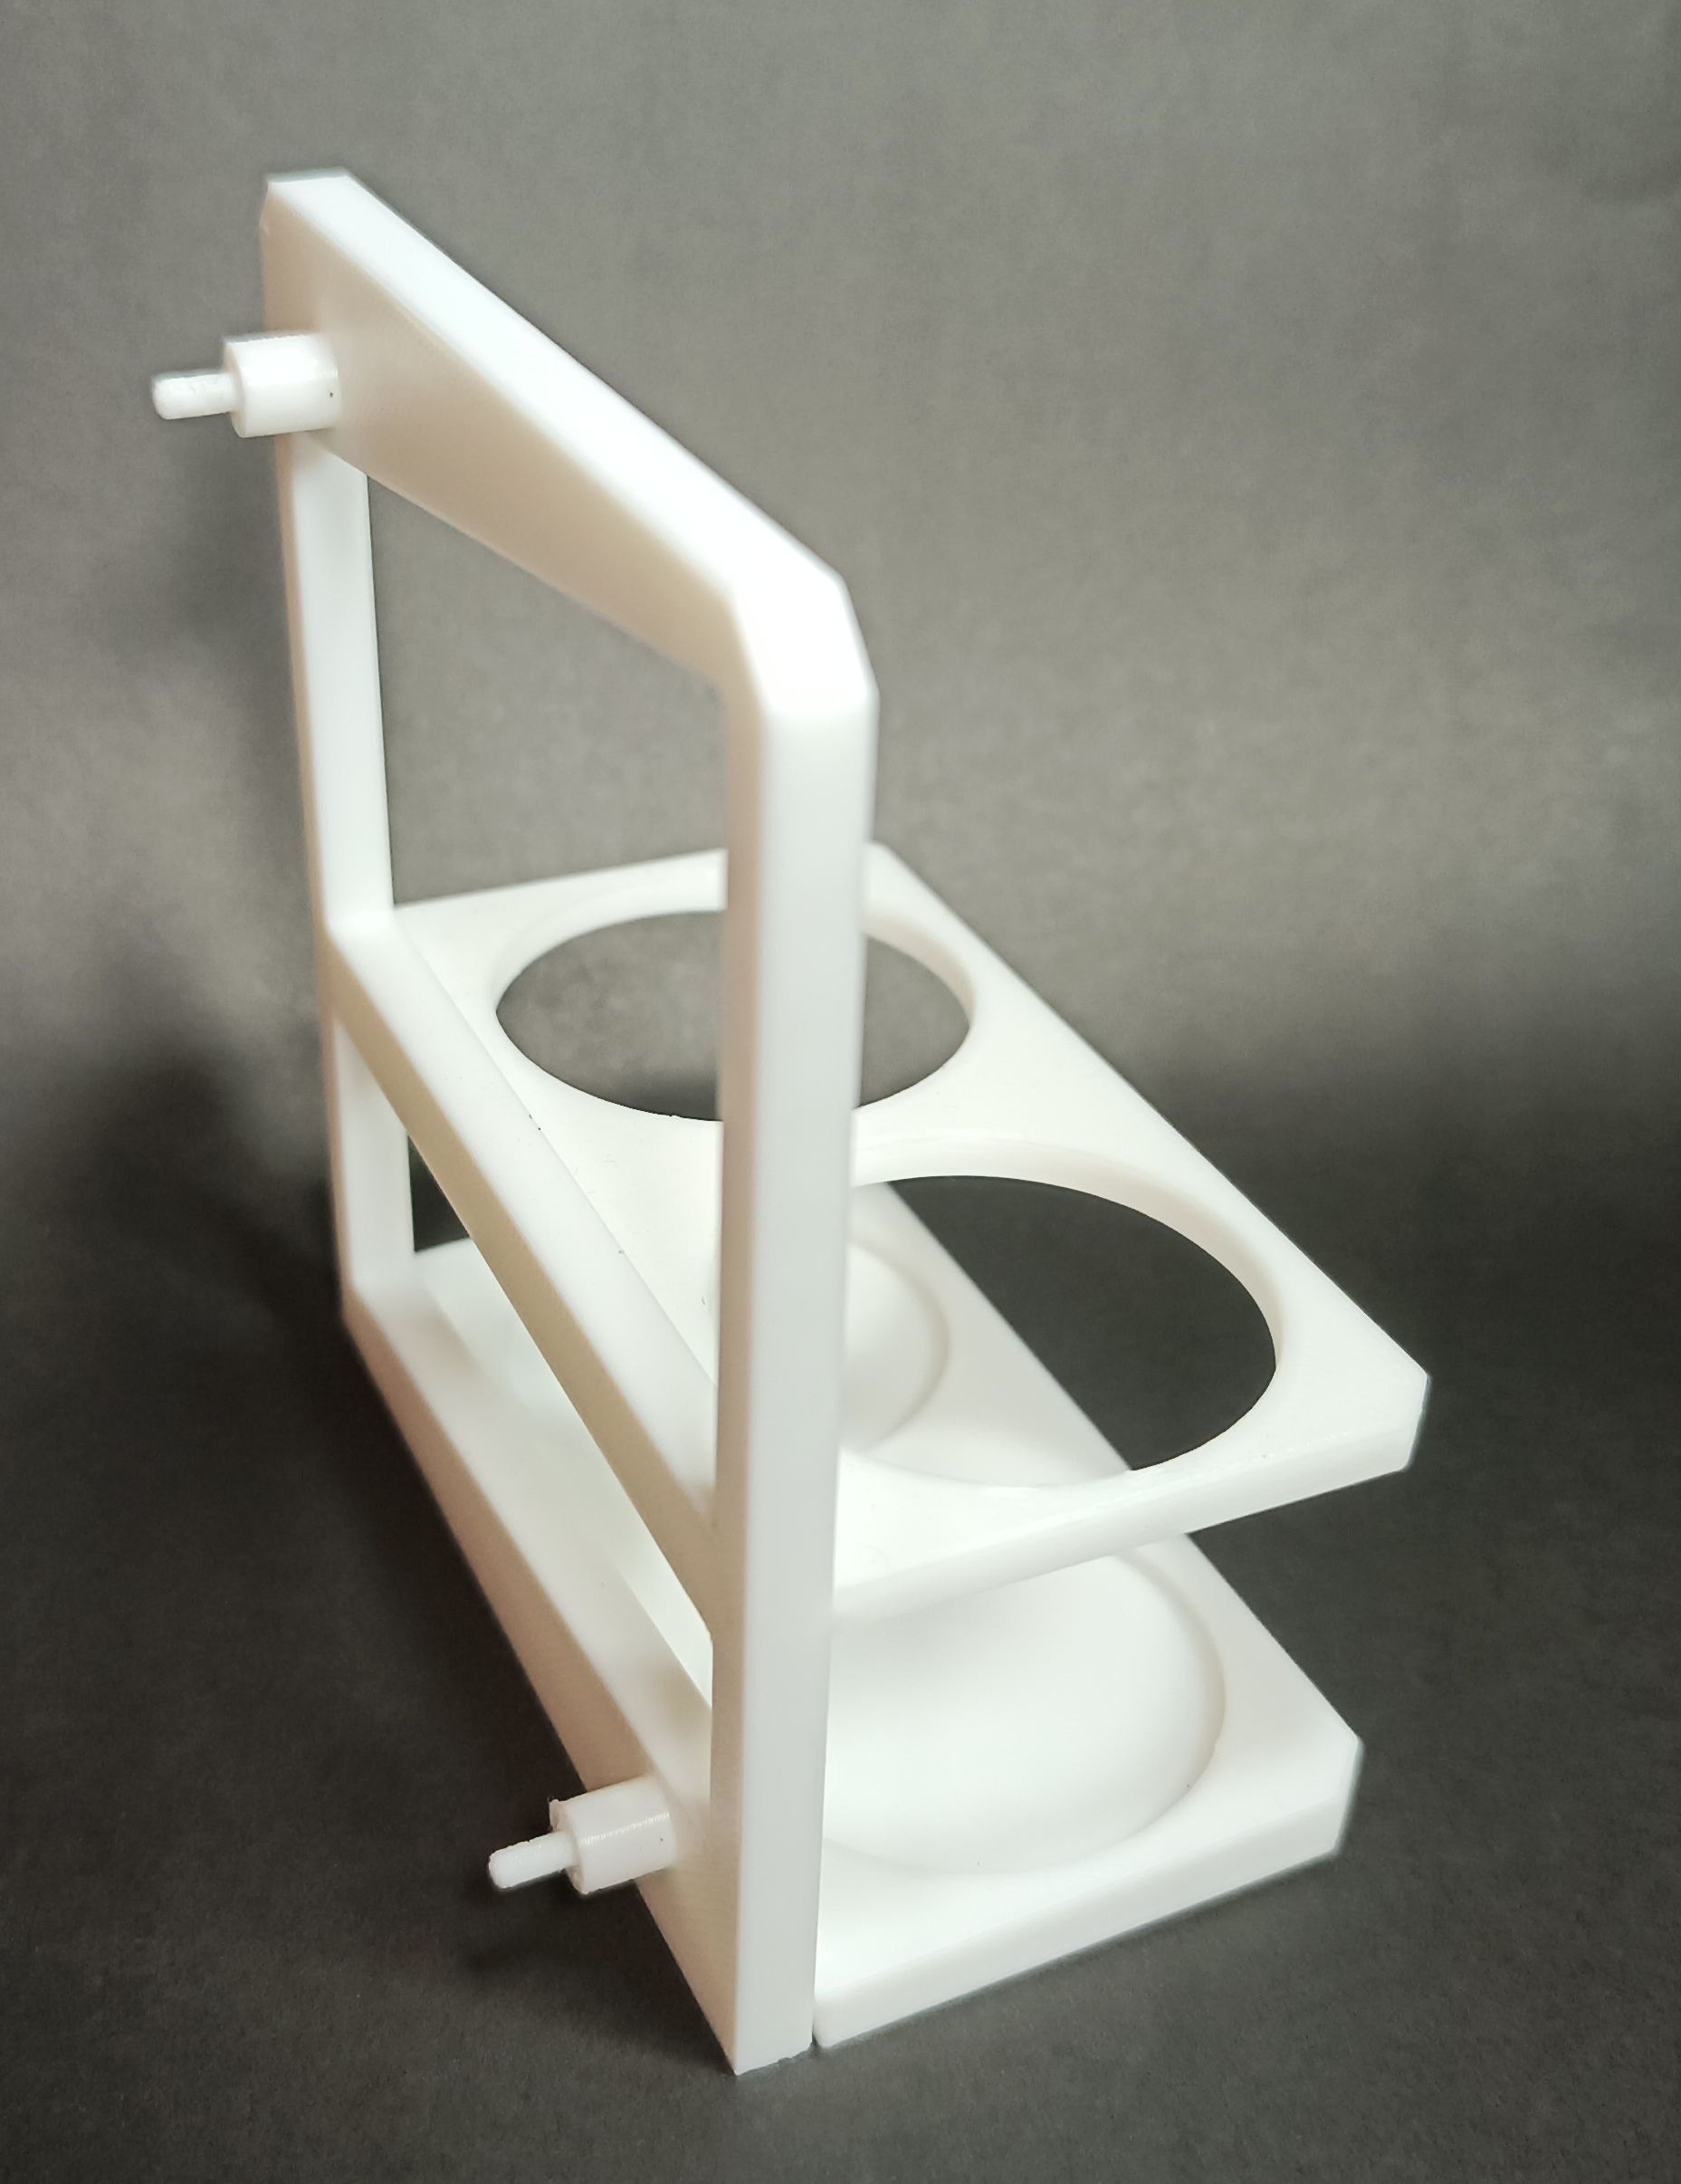
\includegraphics[width=0.9\textwidth]{fig/img/frame_side.png}
    \end{minipage}
    \caption{Rama służąca do podtrzymania płytki drukowanej 
    i~superkondensatorów}
    \label{rys:frame}
\end{figure}

\begin{figure}[H]
    \centering
    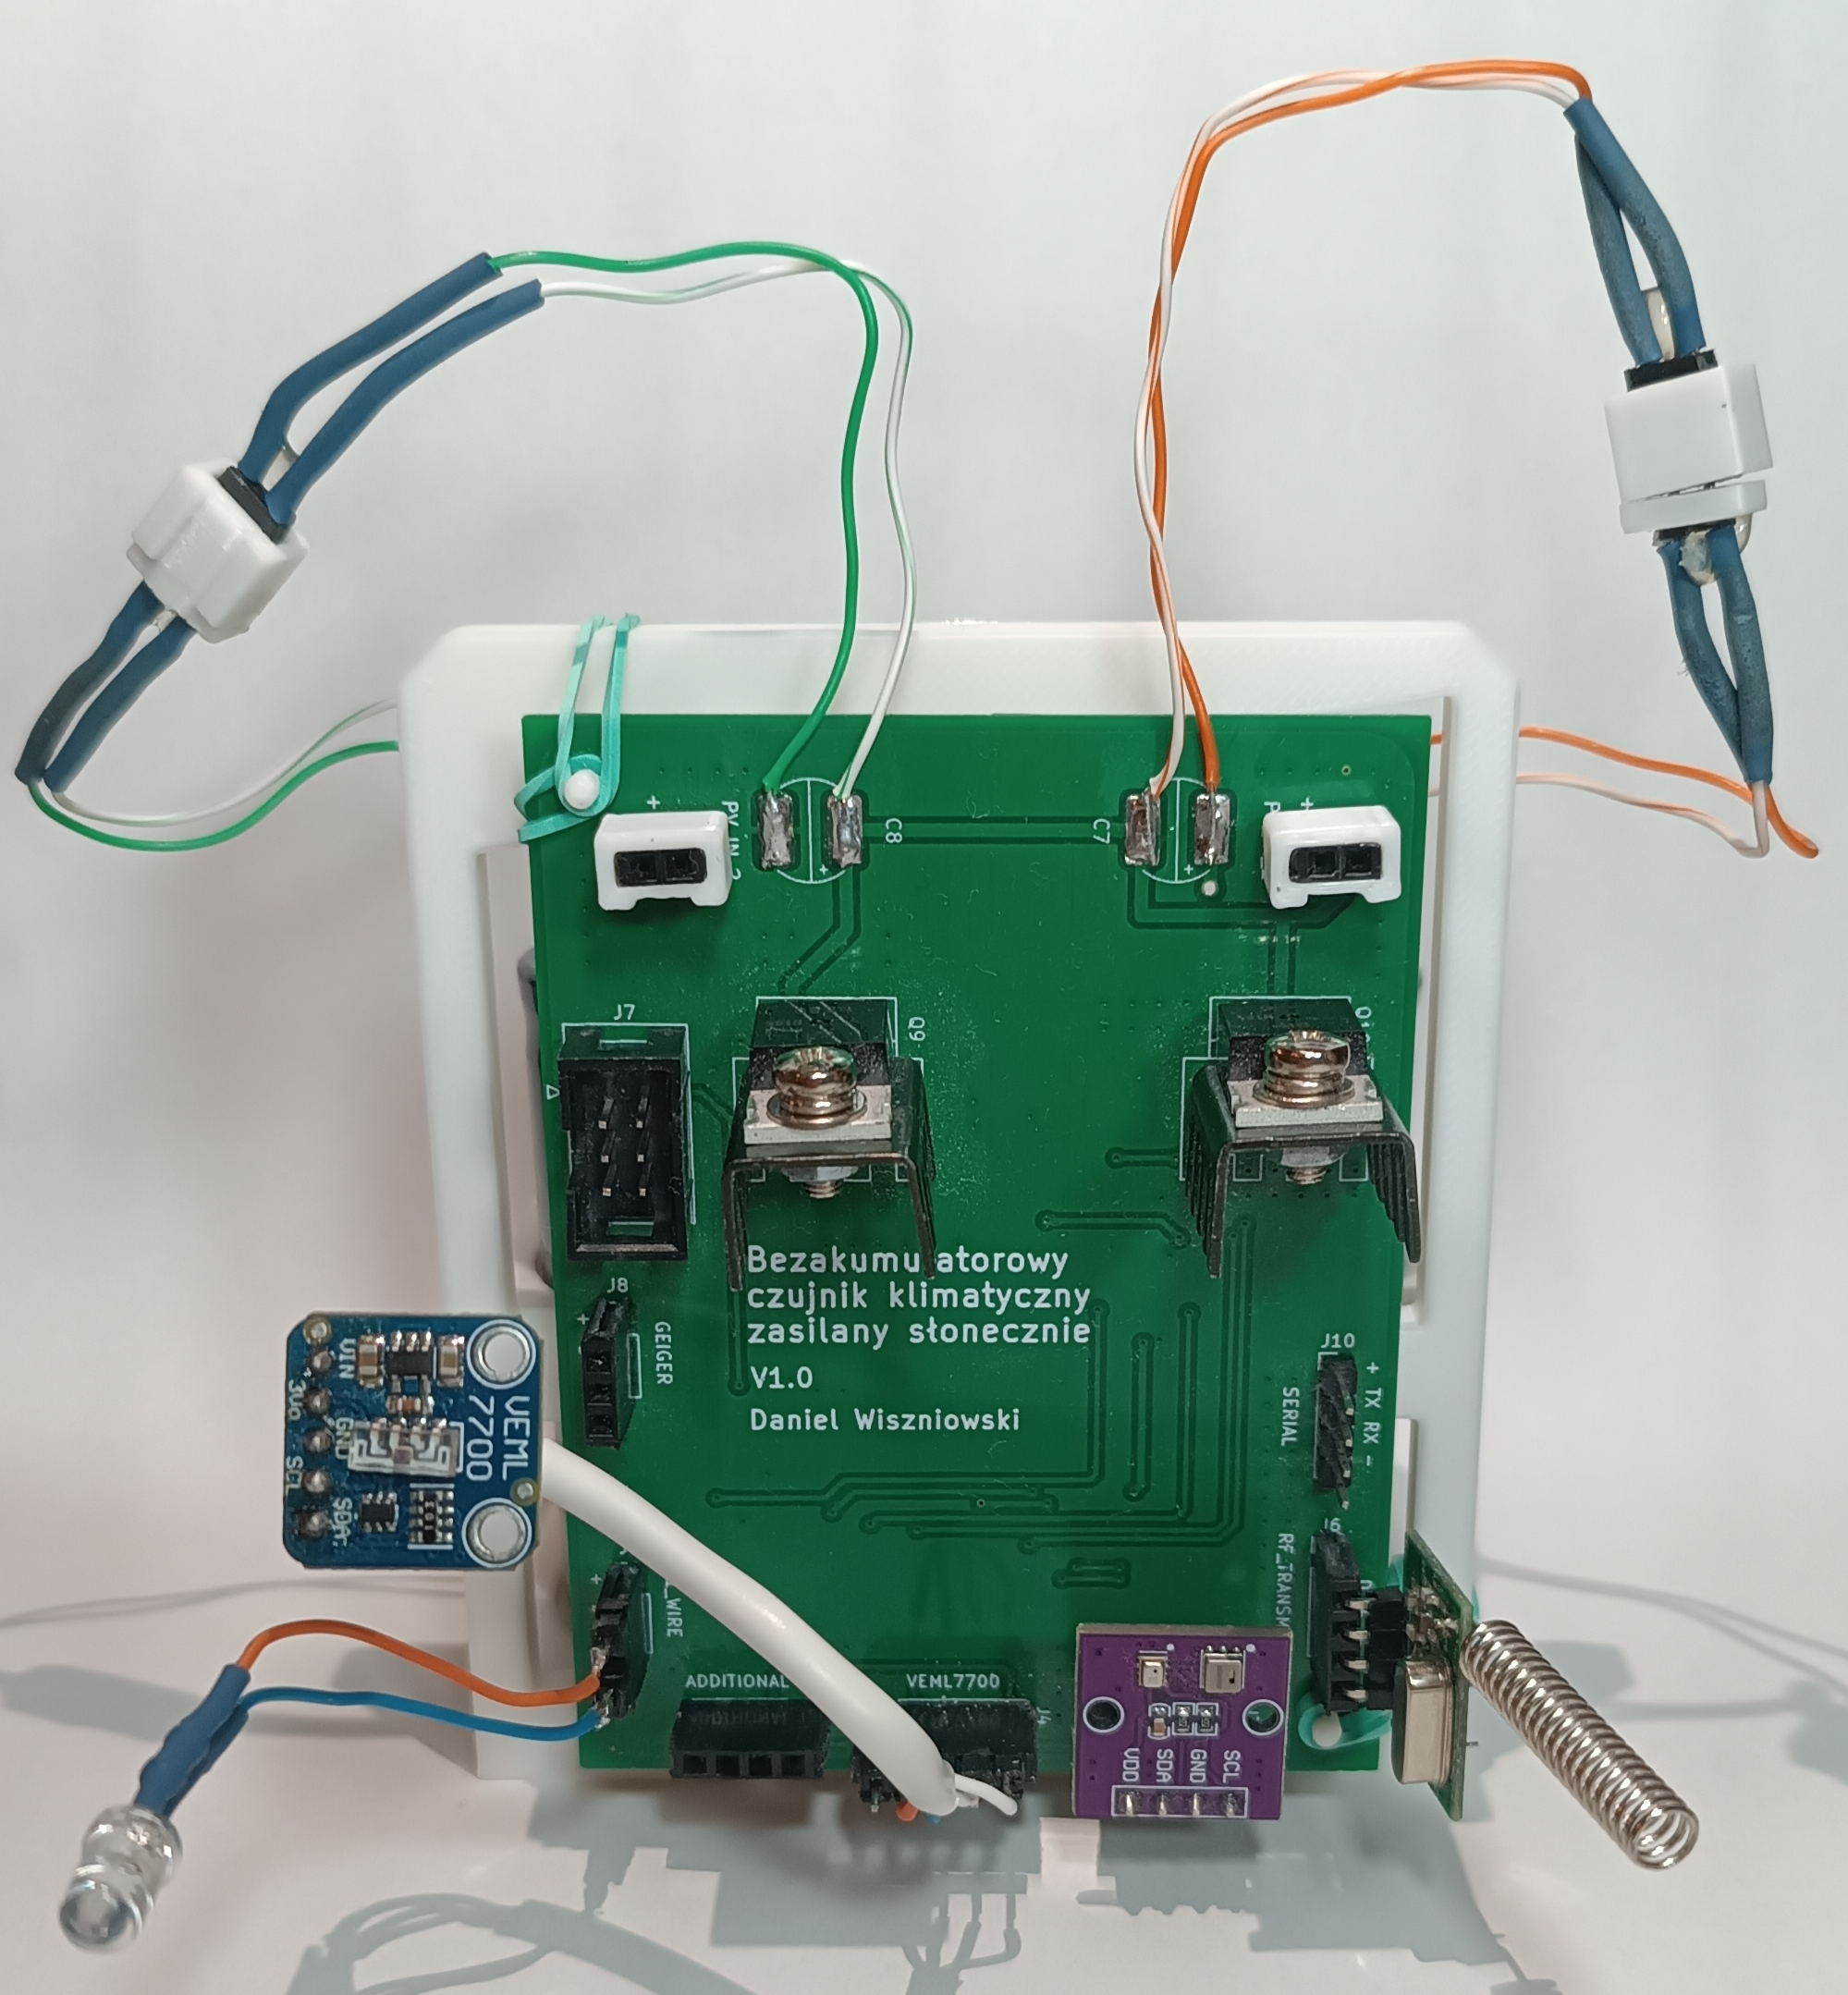
\includegraphics[width=0.9\textwidth]{fig/img/full_test_setup.png}
    \caption{Płytka drukowana uzupełniona o~moduły pomiarowe, nadajnik 
    radiowy oraz diodę statusu umieszczona na ramie i~podłączona do 
    superkondensatorów}
    \label{rys:pcb_on_frame}
\end{figure}

Układ został uzupełniony o~2 monokrystaliczne panele 
fotowoltaiczne. Rysunek~\ref{rys:pv_panel} przedstawia jeden 
z~tych paneli.

\begin{figure}[H]
    \centering
    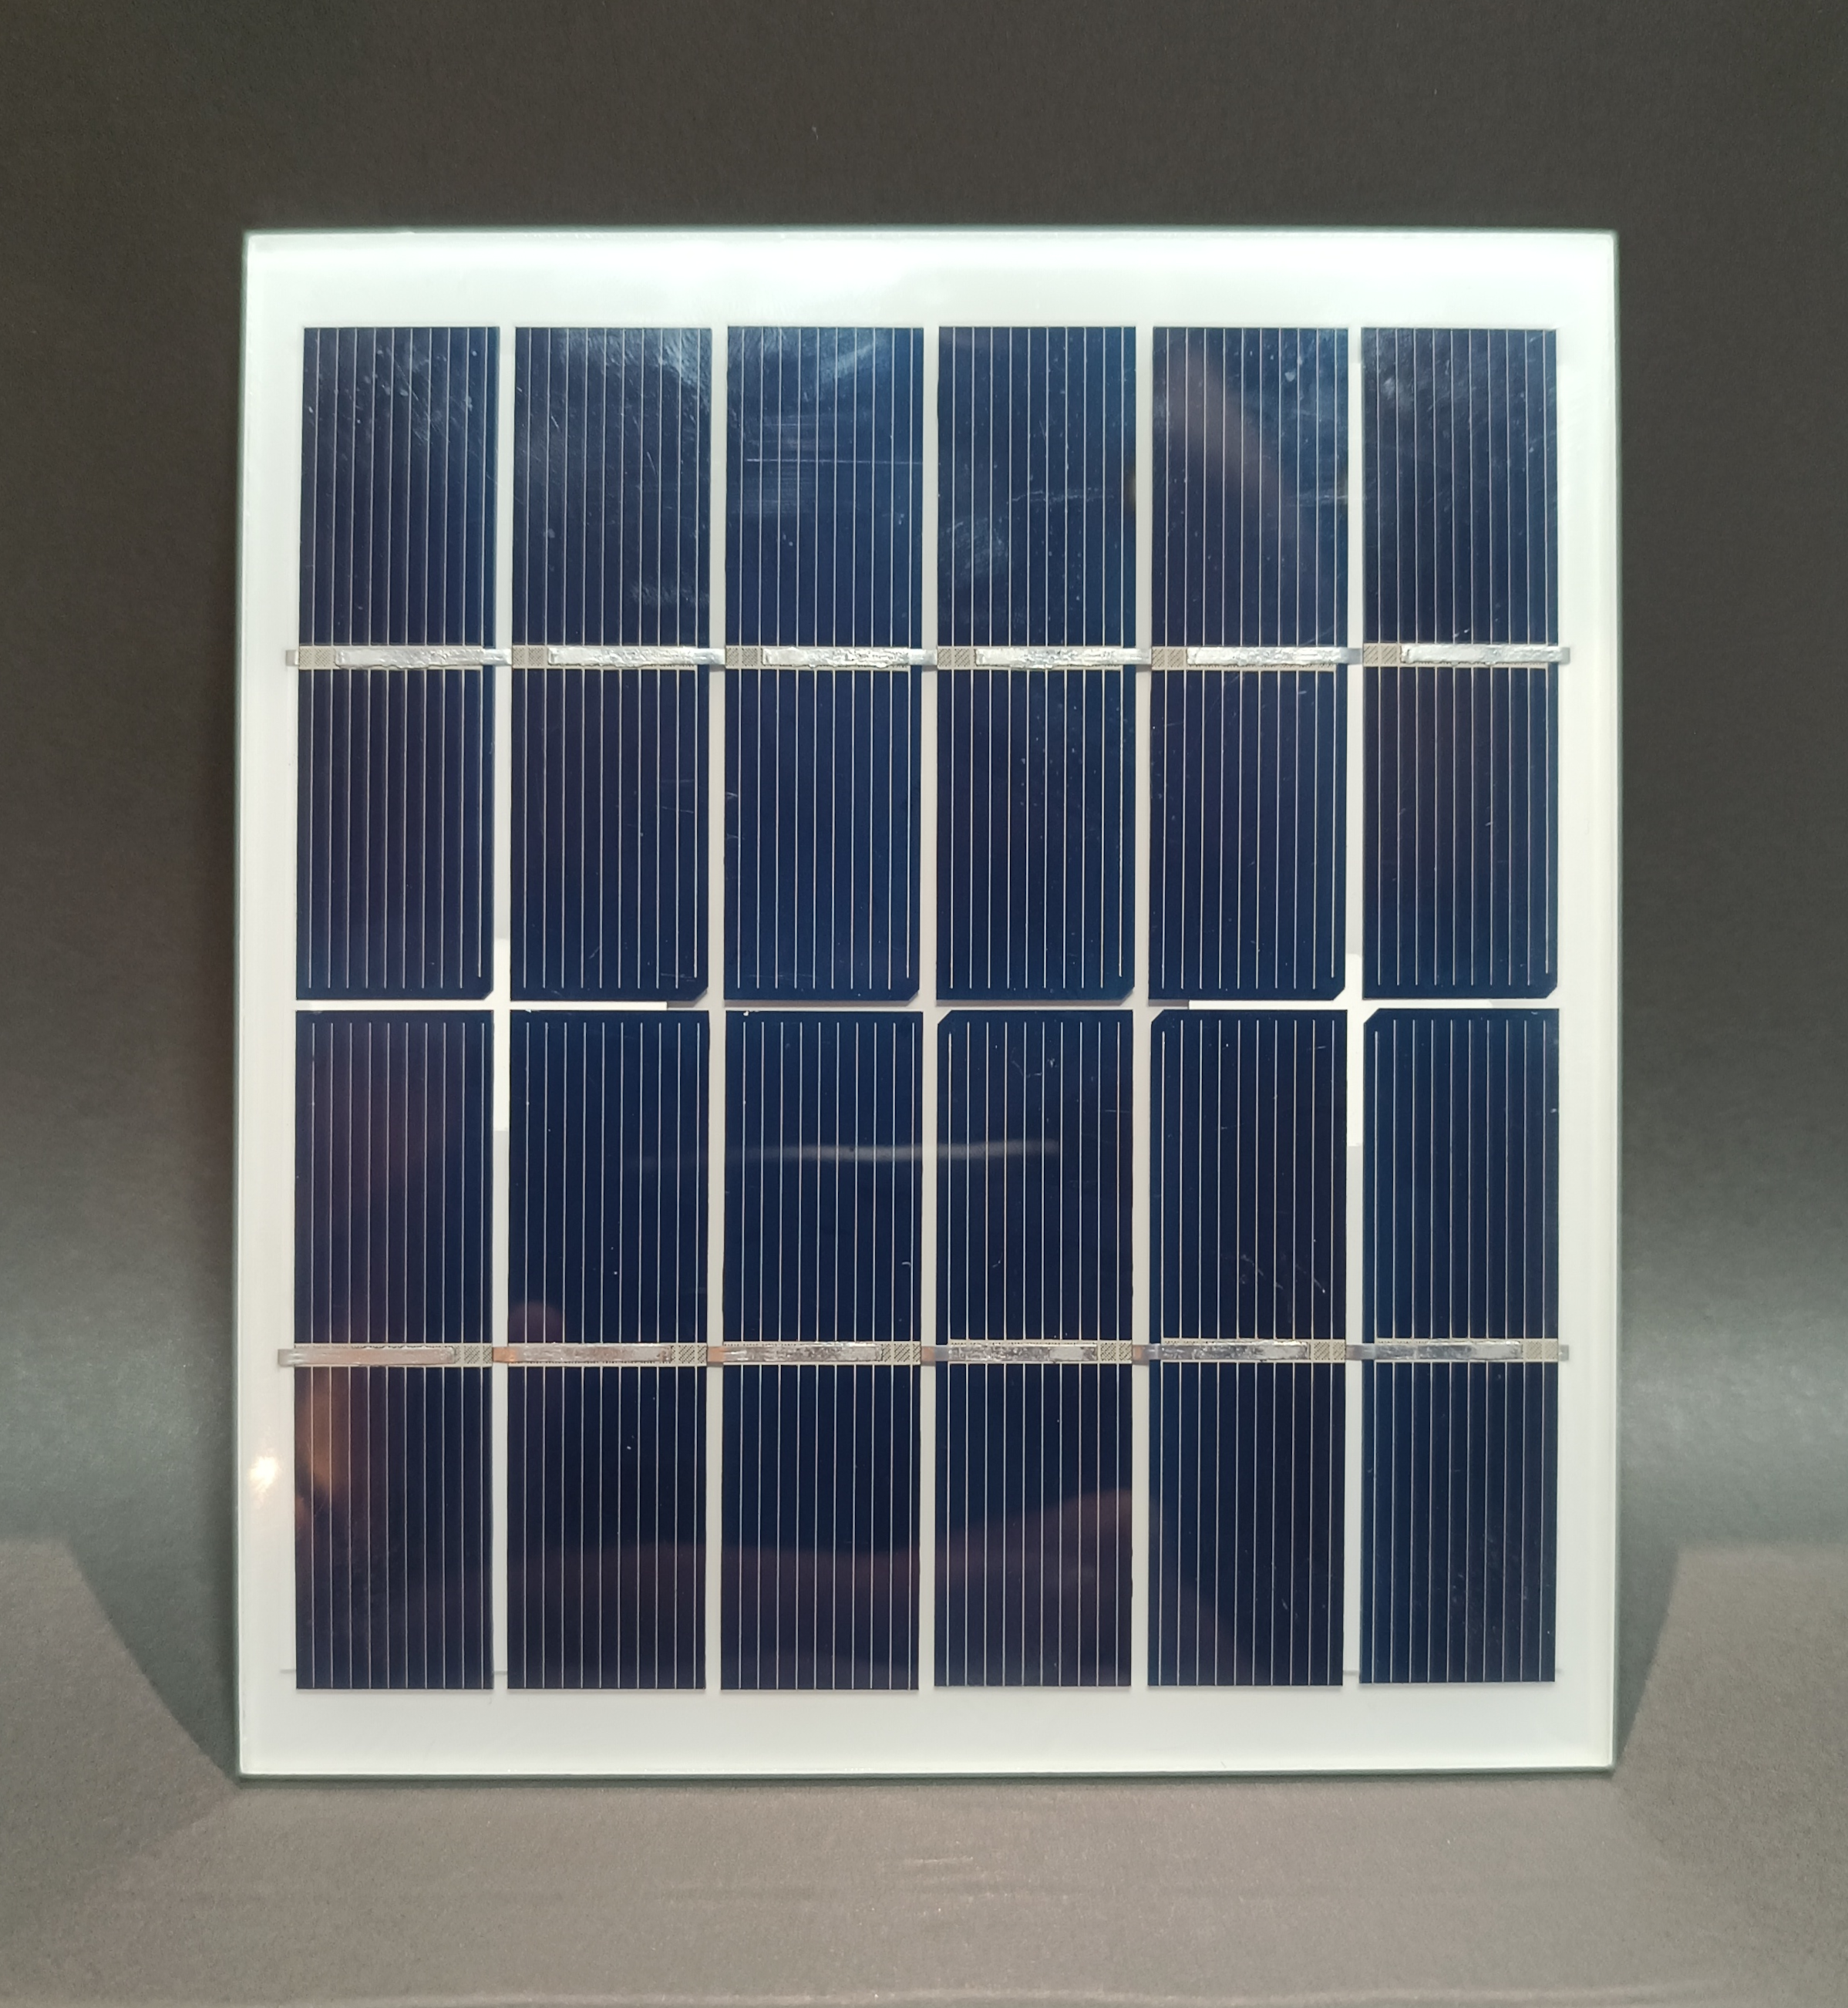
\includegraphics[width=0.9\textwidth]{fig/img/pv_panel.png}
    \caption{Monokrystaliczny panel fotowoltaiczny użyty do zasilenia czujnika
    klimatycznego}
    \label{rys:pv_panel}
\end{figure}

Do odbioru i~przetwarzania danych wysyłanych przez czujnik
klimatyczny wykorzystano odbiornik obsługujący częstotliwość 
\SI{433}{\mega\hertz} podłączony do płytki Arduino NANO.
Arduino NANO przy pomocy autorskiej biblioteki
\texttt{ook\_433mhz} umożliwiało dekodowanie danych odebranych 
od czujnika, a~następnie wysyłanie ich przez port szeregowy 
do komputera, który gromadził je w~pliku CSV.


\section{Przebieg pomiarów}
W~celu przetestowania czujnika klimatycznego w~warunkach
wewnętrznych jak i~zewnętrznych został on poddany
testom trwającym odpowiednio \SI{10}{\hour} i~\SI{31}{\hour},
w~których czujnik wysyłał dane w~jednominutowych
odstępach. Podczas obydwu testów mierzona była 
temperatura, wilgotność względna, ciśnienie atmosferyczne
oraz napięcie na okładkach kondensatorów zasilających.

\subsection*{Pomiary wewnętrzne}
Czujnik funkcjonował poprawnie w~trakcie 10-godzinnego
testu w~warunkach wewnętrznych, trwającego od godziny 
23:58 do godziny 10:42. 
Uzyskane dane pomiarowe to: 
temperatura (rysunek~\ref{rys:graph_temp_ins}),
wilgotność względna (rysunek~\ref{rys:graph_hum_ins}),
ciśnienie atmosferyczne (rysunek~\ref{rys:graph_press_ins}),
natężenie światła (rysunek~\ref{rys:graph_lux_ins})
oraz napięcie na kondensatorach (rysunek~\ref{rys:graph_volt_ins}).

W~celu wykonania tego testu czujnik klimatyczny został 
umieszczony z~dala od źródeł ciepła i~światła. Panele
fotowoltaiczne również były umieszczone w~dużej odległości
od bezpośredniego światła słonecznego.

\begin{figure}[H]
    \centering
    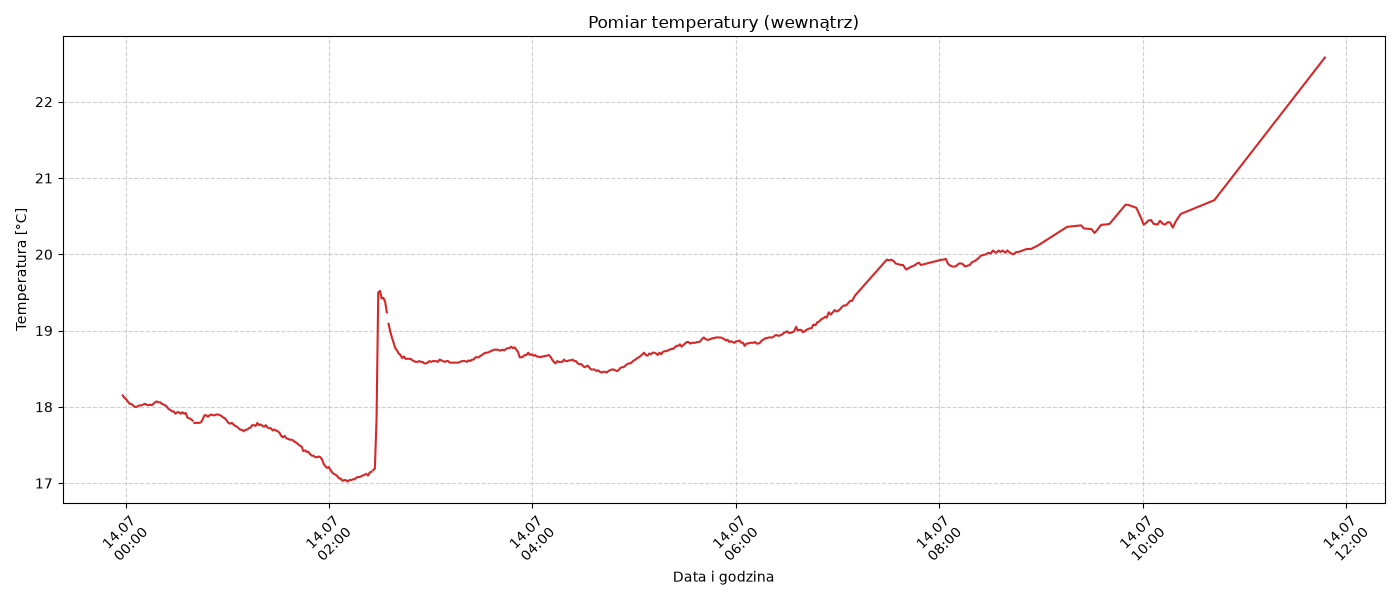
\includegraphics[width=0.9\textwidth]{fig/graphs/temperatura_inside.png}
    \caption{Wykres przedstawiający pomiary wartości temperatury w~warunkach wewnętrznych}
    \label{rys:graph_temp_ins}
\end{figure}

\begin{figure}[H]
    \centering
    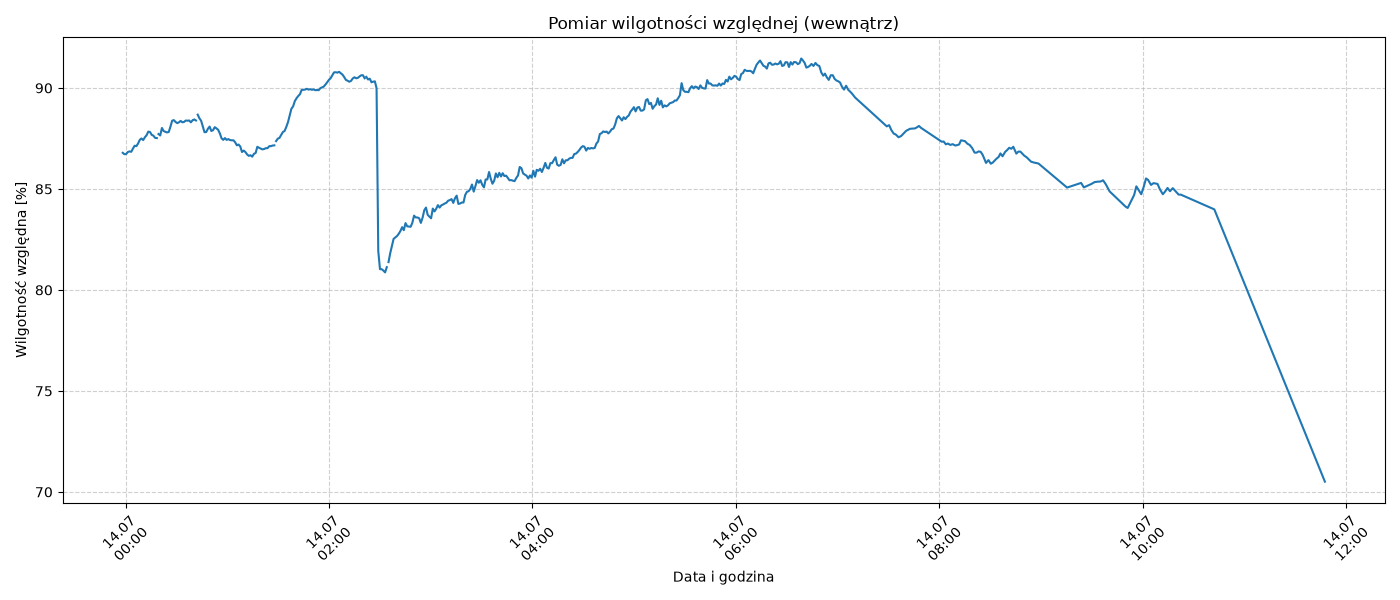
\includegraphics[width=0.9\textwidth]{fig/graphs/humidity_inside.png}
    \caption{Wykres przedstawiający pomiary wartości wilgotności względnej w~warunkach wewnętrznych}
    \label{rys:graph_hum_ins}
\end{figure}

\begin{figure}[H]
    \centering
    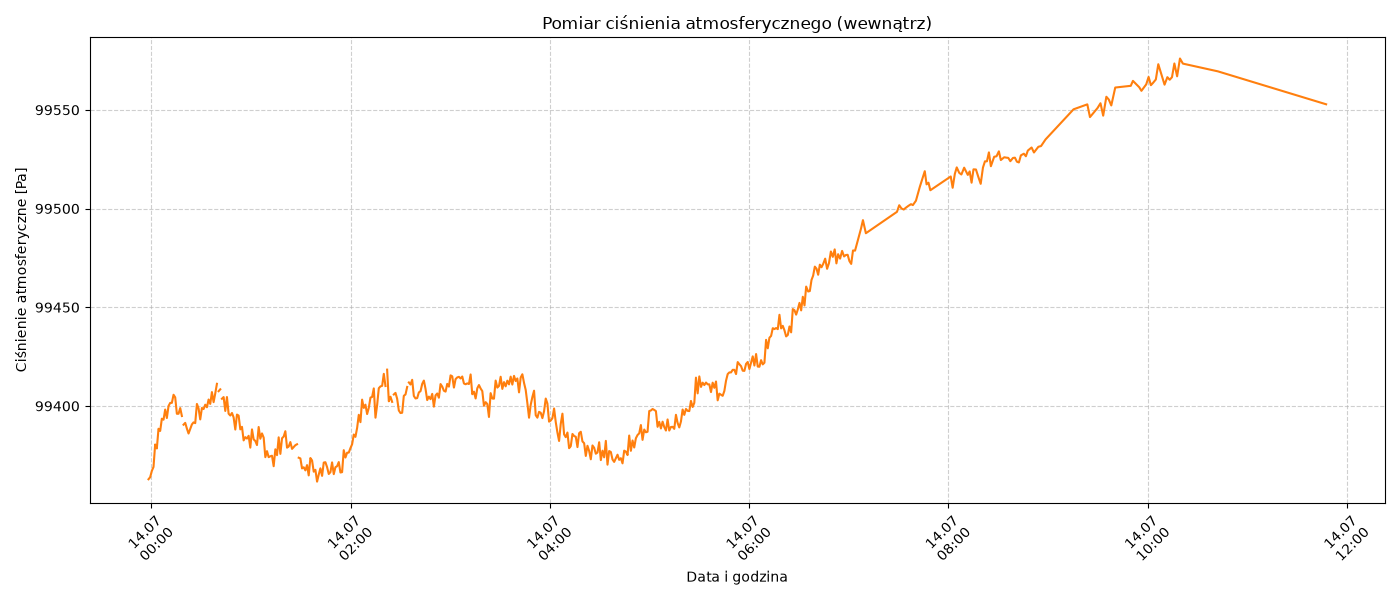
\includegraphics[width=0.9\textwidth]{fig/graphs/pressure_inside.png}
    \caption{Wykres przedstawiający pomiary wartości ciśnienia atmosferycznego w~warunkach wewnętrznych}
    \label{rys:graph_press_ins}
\end{figure}

\begin{figure}[H]
    \centering
    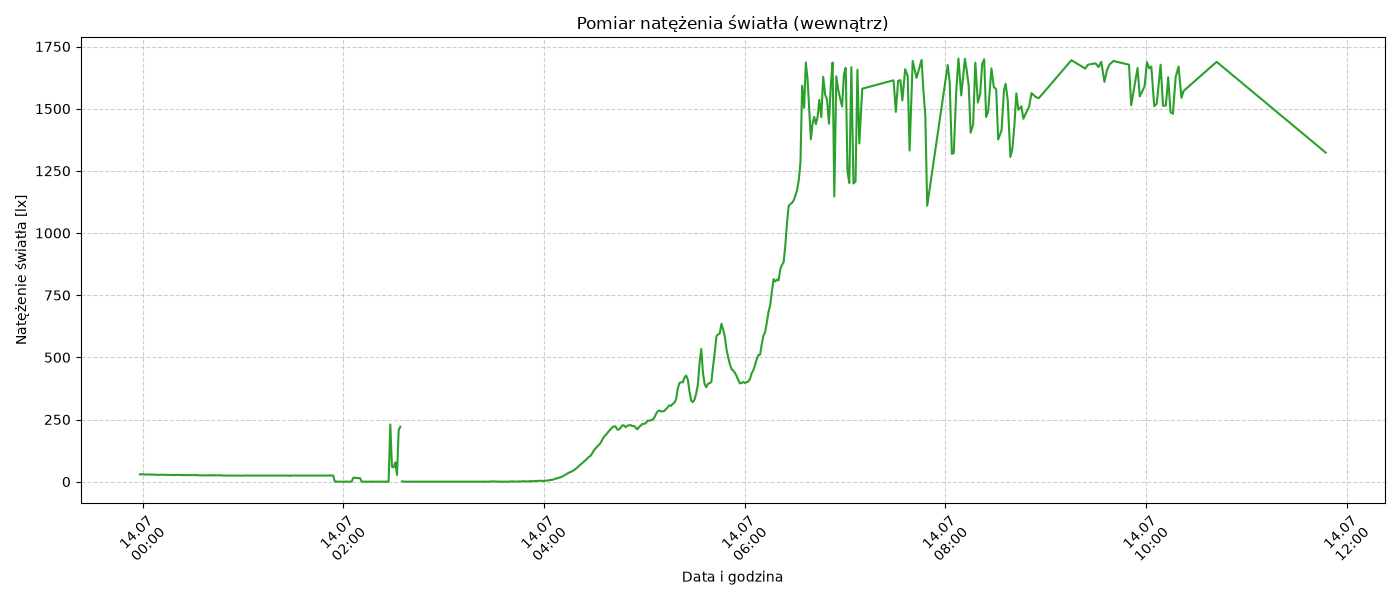
\includegraphics[width=0.9\textwidth]{fig/graphs/lux_inside.png}
    \caption{Wykres przedstawiający pomiary wartości natężenie światła w~warunkach wewnętrznych}
    \label{rys:graph_lux_ins}
\end{figure}

\begin{figure}[H]
    \centering
    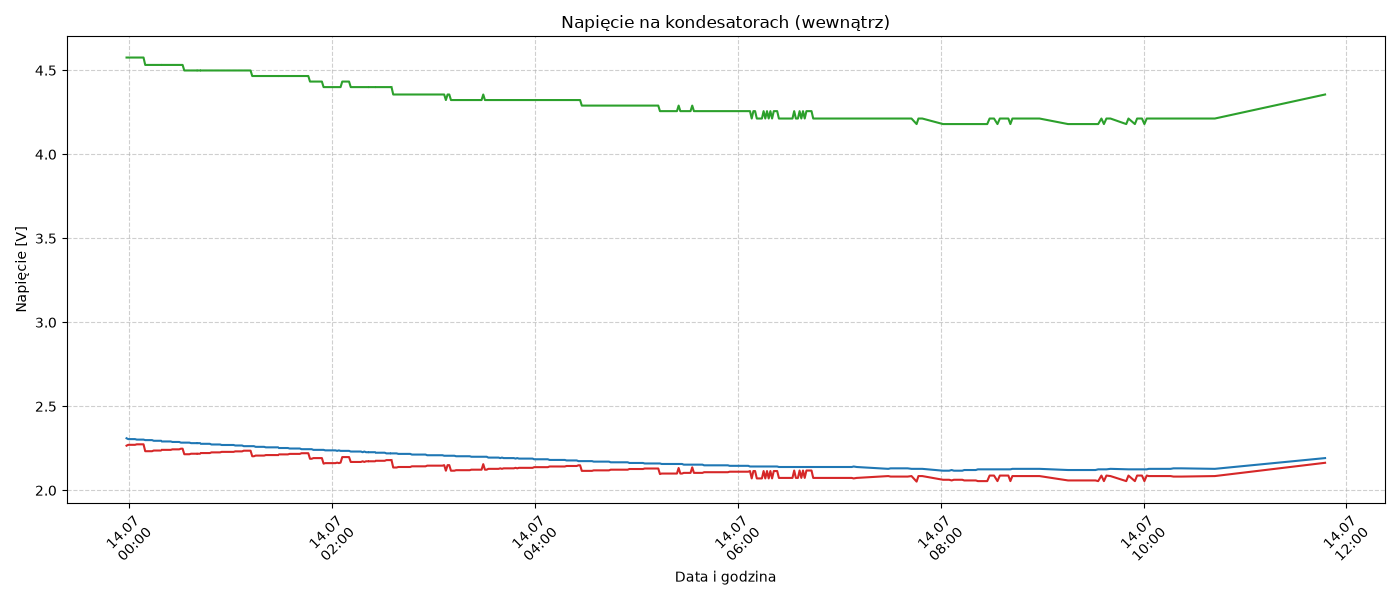
\includegraphics[width=0.9\textwidth]{fig/graphs/voltage_inside.png}
    \caption{Wykres przedstawiający pomiary wartości napięcia na okładkach kondensatorów w~warunkach wewnętrznych}
    \label{rys:graph_volt_ins}
\end{figure}


\subsection*{Pomiary zewnętrzne}
Podobnie, jak w~przypadku pomiarów wewnętrznych, nie 
odnotowano zakłóceń w~pracy czujnika klimatycznego. Test trwał
od godziny 15:28 dnia 14 lipca, do godziny 22:25 dnia 
następnego. Zebrane w~tym czasie dane zostały przedstawione
na wykresach: 
temperatury (rysunek~\ref{rys:graph_temp}),
wilgotności względnej (rysunek~\ref{rys:graph_hum}),
ciśnienia atmosferycznego (rysunek~\ref{rys:graph_press}),
natężenia światła (rysunek~\ref{rys:graph_lux})
oraz napięcia na kondensatorach (rysunek~\ref{rys:graph_volt}).

Do przeprowadzenia tego testu czujnik klimatyczny (jak i~panele 
fotowoltaiczne) znajdował się w~cieniu, na skierowanej na 
południowy zachód ścianie domu. Taka lokalizacja nie zapewniała
optymalnych warunków nasłonecznienia paneli fotowoltaicznych.

\begin{figure}[H]
    \centering
    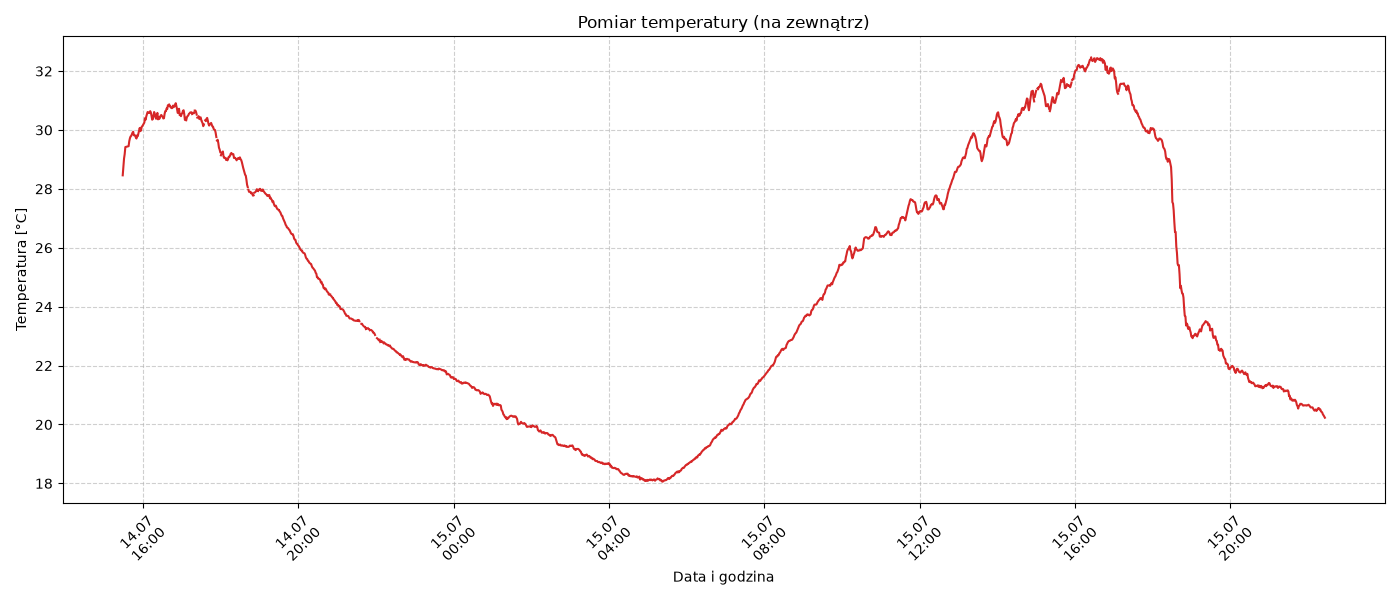
\includegraphics[width=0.9\textwidth]{fig/graphs/temperatura.png}
    \caption{Wykres przedstawiający pomiary wartości temperatury w~warunkach zewnętrznych}
    \label{rys:graph_temp}
\end{figure}

\begin{figure}[H]
    \centering
    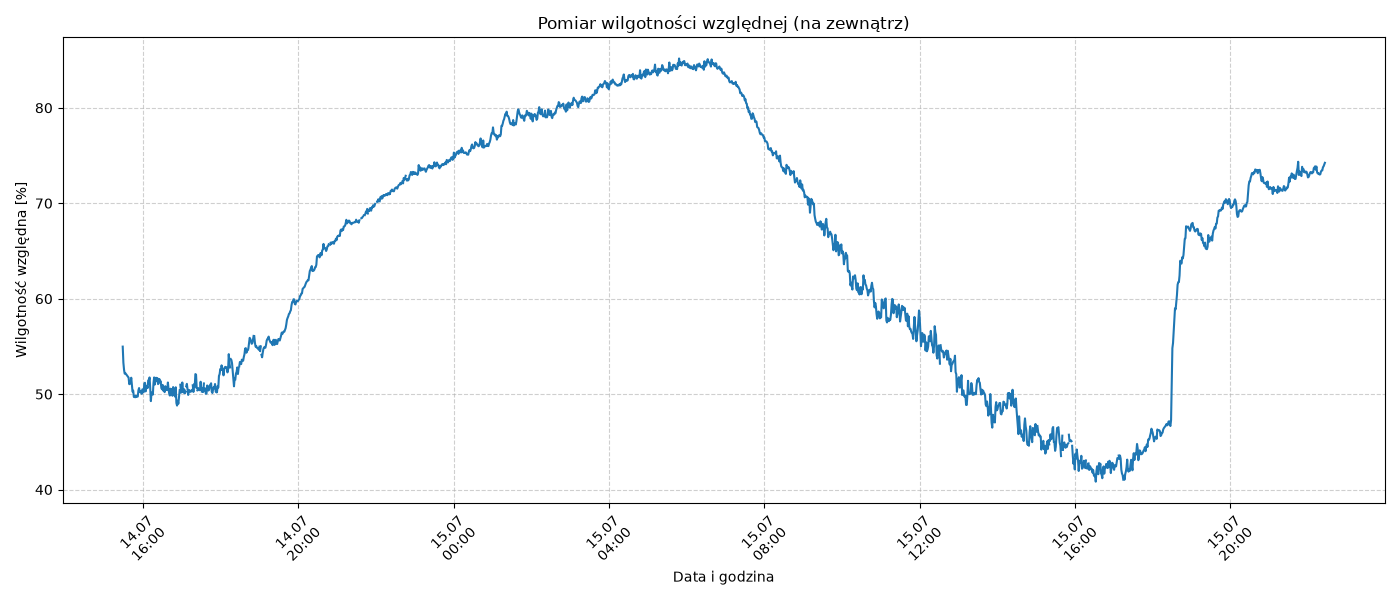
\includegraphics[width=0.9\textwidth]{fig/graphs/humidity.png}
    \caption{Wykres przedstawiający pomiary wartości wilgotności względnej w~warunkach zewnętrznych}
    \label{rys:graph_hum}
\end{figure}

\begin{figure}[H]
    \centering
    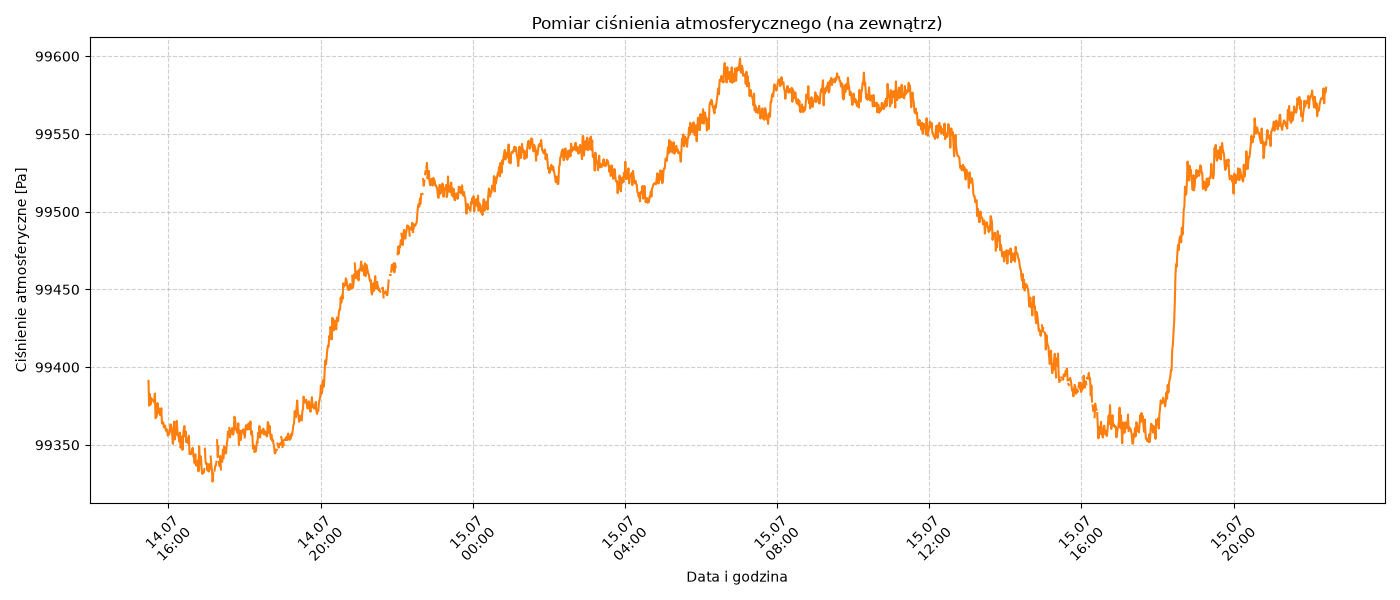
\includegraphics[width=0.9\textwidth]{fig/graphs/pressure.png}
    \caption{Wykres przedstawiający pomiary wartości ciśnienia atmosferycznego w~warunkach zewnętrznych}
    \label{rys:graph_press}
\end{figure}

\begin{figure}[H]
    \centering
    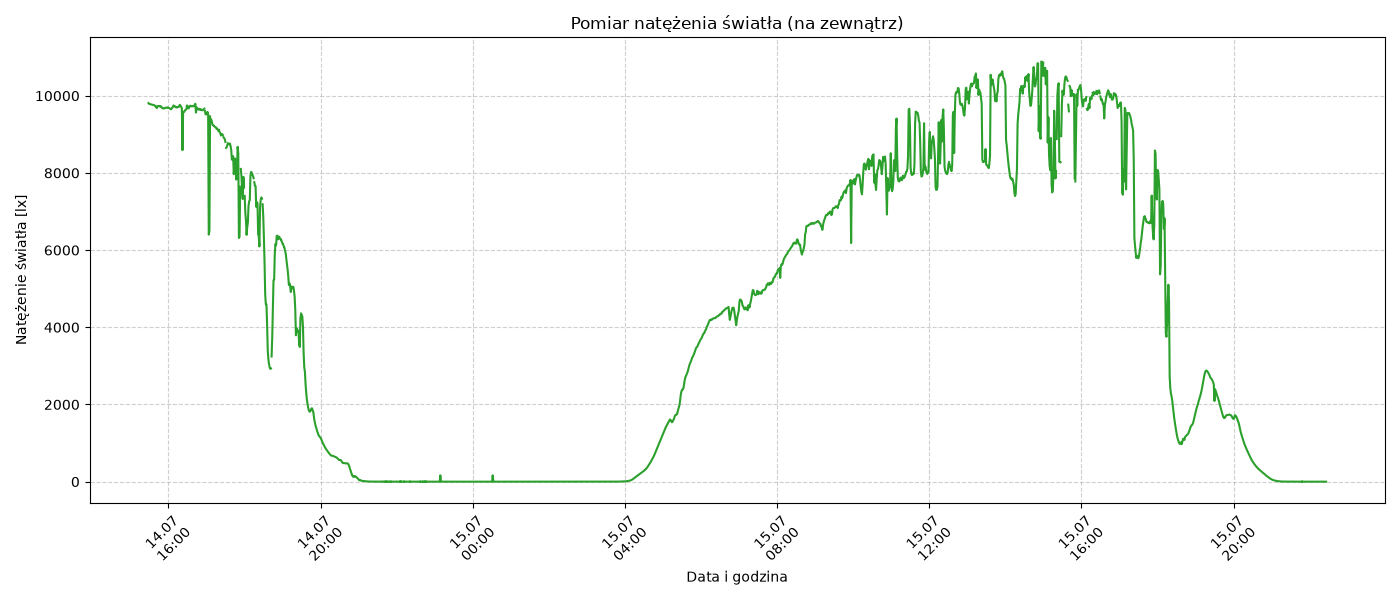
\includegraphics[width=0.9\textwidth]{fig/graphs/lux.png}
    \caption{Wykres przedstawiający pomiary wartości natężenie światła w~warunkach zewnętrznych}
    \label{rys:graph_lux}
\end{figure}

\begin{figure}[H]
    \centering
    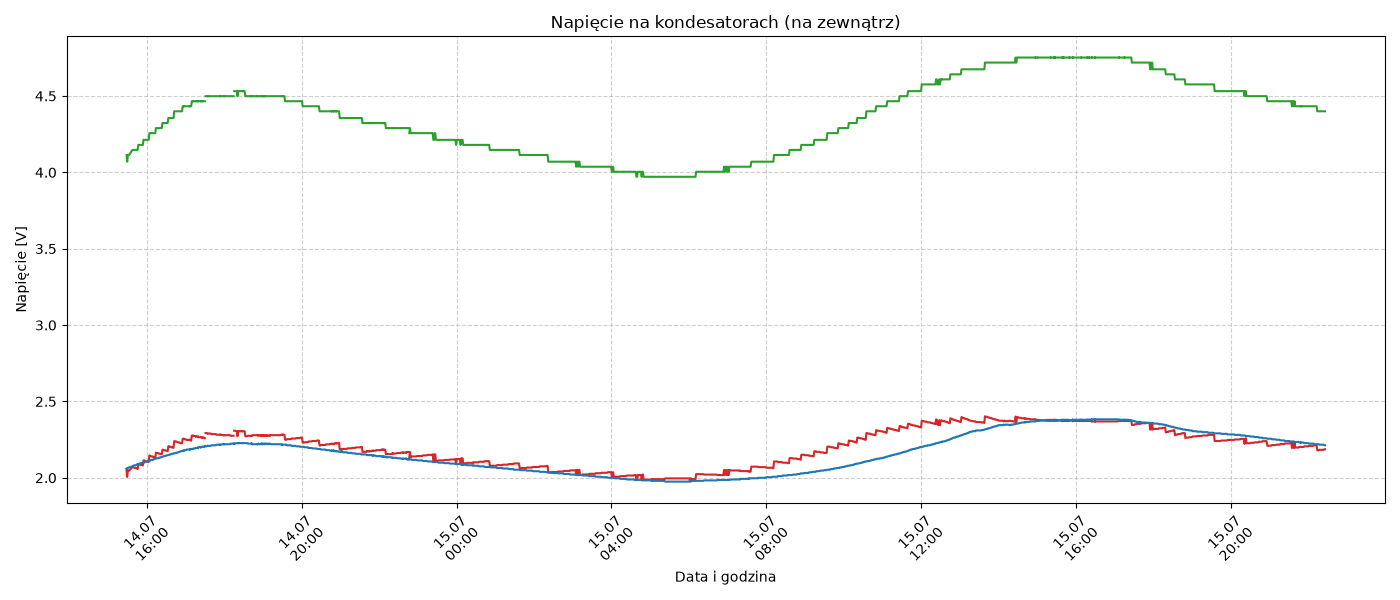
\includegraphics[width=0.9\textwidth]{fig/graphs/voltage.png}
    \caption{Wykres przedstawiający pomiary wartości napięcia na okładkach kondensatorów w~warunkach zewnętrznych}
    \label{rys:graph_volt}
\end{figure}


\section{Wnioski}
Utworzony na potrzeby tego projektu czujnik klimatyczny 
może być stosowany zarówno w~warunkach wewnętrznych, 
jak i~zewnętrznych. 

W~przypadku użycia czujnika na zewnątrz panele fotowoltaiczne 
umożliwiają naładowanie superkondensatorów w~ciągu dnia, nawet przy 
braku bezpośrednio padającego na nie światła słonecznego.
Natomiast w~przypadku użycia wewnętrznego koniecznym może być
ustawienie paneli bliżej bezpośredniego źródła światła słonecznego. 

Zgromadzony w~superkondensatorach ładunek pozwala na 
podtrzymanie pracy urządzenia przez okres 12 godzin, 
rozładowując się w~tym czasie do sumarycznej wartości 
\SI{4}{\volt}, pozostawiając~\SI{3}{\volt} zapasu.